\documentclass[11pt,a4paper]{article}

\usepackage[utf8]{inputenc}
\usepackage[english]{babel}
\usepackage[T1]{fontenc}
\usepackage{lmodern}
\usepackage{mathtools}
\usepackage{subcaption}
\usepackage{float}

\usepackage{amsmath,amssymb,amsfonts}

\DeclarePairedDelimiter{\ceil}{\lceil}{\rceil}
\DeclarePairedDelimiter{\floor}{\lfloor}{\rfloor}

\title{Vision and Image Processing\\Assignment 1}
\author{Malte Stær Nissen}

\begin{document}
\maketitle

\section{Detecting interest points}

The detection of interest points can be made by utilizing a variety of methods. I
have implemented\footnote{The entire implementation of this assignment is made
in Matlab 2012b.} both the two blob detectors Difference of Gaussians (DoG) and
Laplacian of Gaussian (LoG) as well as the Harris corner detector. All three detectors
are implemented by hand only using simple Matlab standard functions.

\subsection{Blob detectors}

Both blob detectors are implemented by first creating either a DoG or LoG
filter. These filters are created by sampling the appropriate Gaussian
distribution(s) (and their derrivatives) with a support radius of $3\sigma$
and hence a filter size of $\ceil{6 \sigma} \times \ceil{6\sigma}$ in order to
get a sufficient part of the distribution included in the filter. The second
part of the blob detectors is to perform a simple convolution of an image with
the filter just found. The boundary cases are handled by using replication of
boundary pixels to avoid the padding to contribute to the derrivatives. The
third and last part of the blob detectors is to find local extrema in
the convolved image using either 4- or 8-connectivity and leave out extremas
below a certain threshold.

\subsection{Harris corner detector}
The Harris corner detector is likewise implemented by computing derrivatives of
the Gaussian distribution, filtering appropriately and then computing the Harris
corner measure followed by a local maxima search and thresholding.

\subsection{Results and parameters}
Figure \ref{fig:i1_points} shows the 50 most significant interest points of running each
of the three point detectors on the image
\texttt{Img\_001\_diffuse\_smallgray.png}. The red crosses, green circles and
yellow squares mark the LoG, DoG and Harris results respectively. The LoG and
DoG points are selected by choosing the 25 most significant light and dark
points. The selection of points is however only made in order to visually
determine the outcome of the algorithms.
\begin{figure}[H]
    \centering
    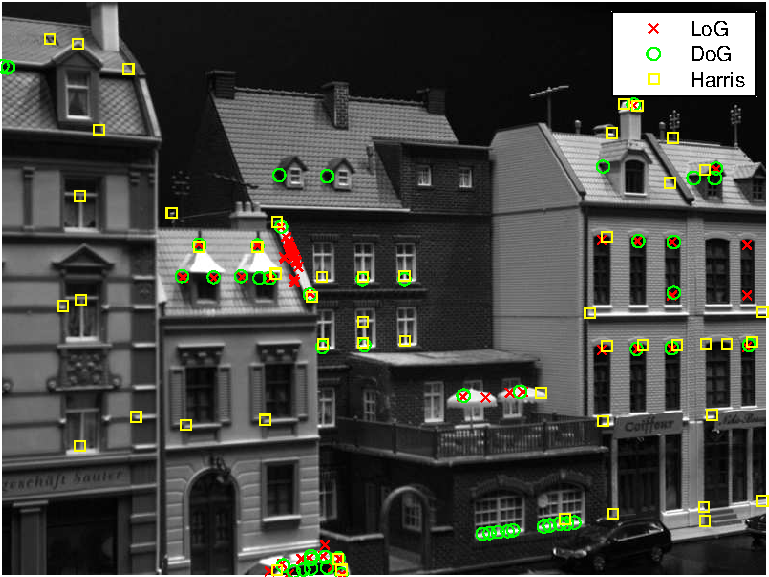
\includegraphics[width=\textwidth]{images/i1_points.pdf}
    \caption{Plot of the 50 most signification interest points in
        \texttt{Img\_001\_diffuse\_smallgray.png} using the
    LoG (red crosses), DoG (green circles), and Harris (yellow squares)
detector.}
    \label{fig:i1_points}
\end{figure}

\section{Simple matching of features}

\begin{figure}[H]
    \begin{subfigure}[t]{\textwidth}
        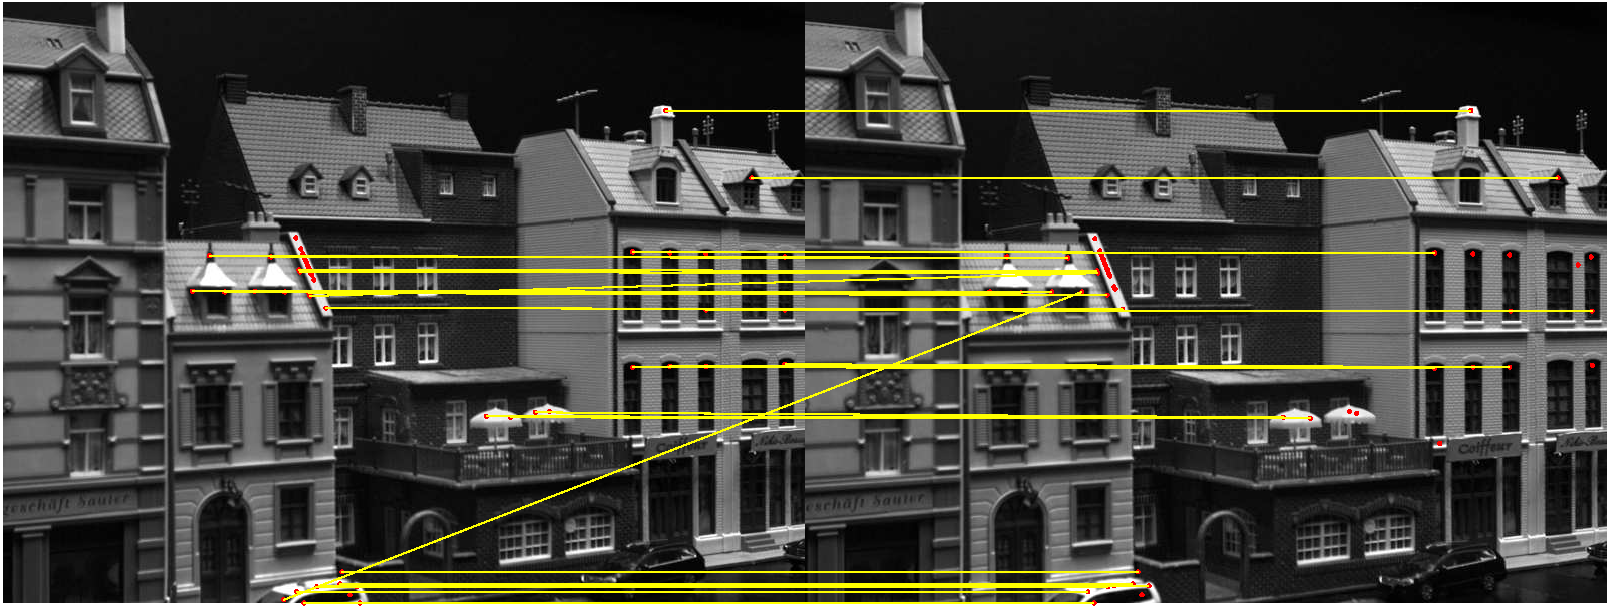
\includegraphics[width=\textwidth]{images/match_i1_i2_log.pdf}
        \caption{LoG points matched between I1 and I2}
        \label{fig:i1_i2_log}
    \end{subfigure}
    \begin{subfigure}[t]{\textwidth}
        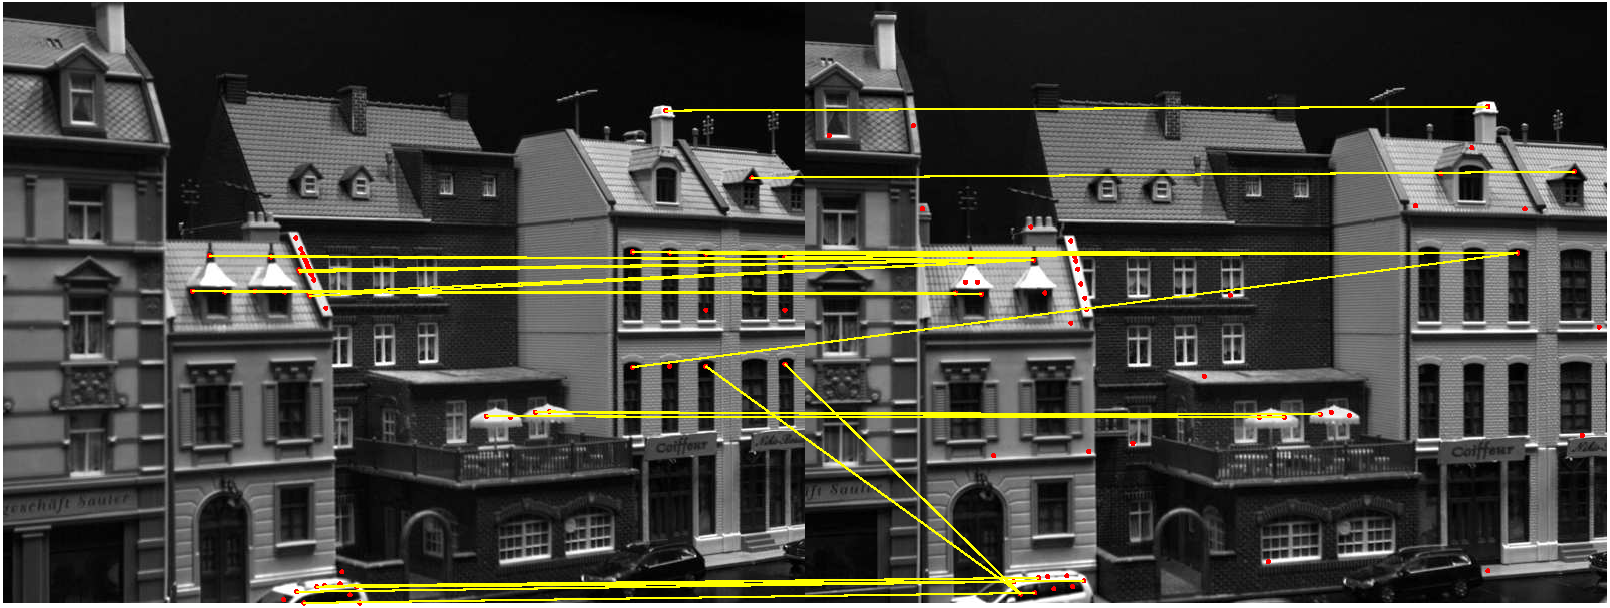
\includegraphics[width=\textwidth]{images/match_i1_i3_log.pdf}
        \caption{LoG points matched between I1 and I3}
        \label{fig:i1_i3_log}
    \end{subfigure}
\end{figure}
\begin{figure}[H]
    \begin{subfigure}[t]{\textwidth}
        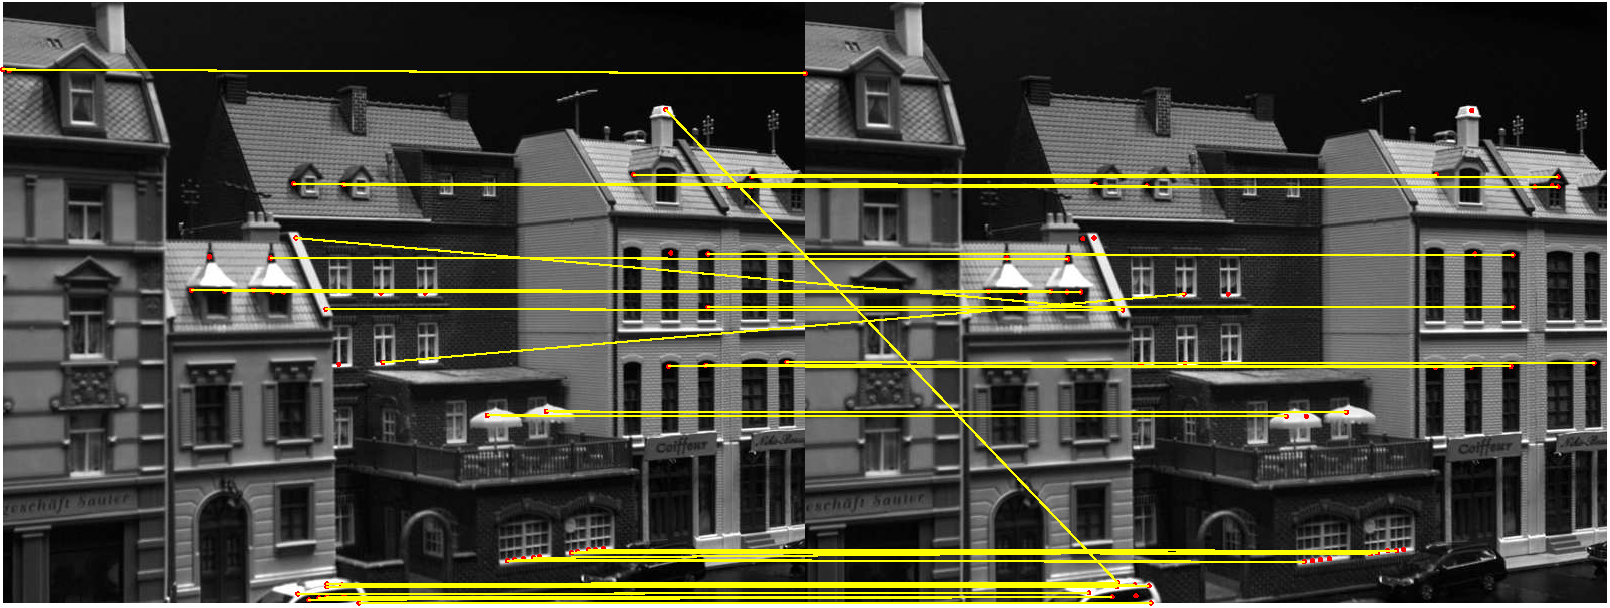
\includegraphics[width=\textwidth]{images/match_i1_i2_dog.pdf}
        \caption{DoG points matched between I1 and I2}
        \label{fig:i1_i2_dog}
    \end{subfigure}
    \begin{subfigure}[t]{\textwidth}
        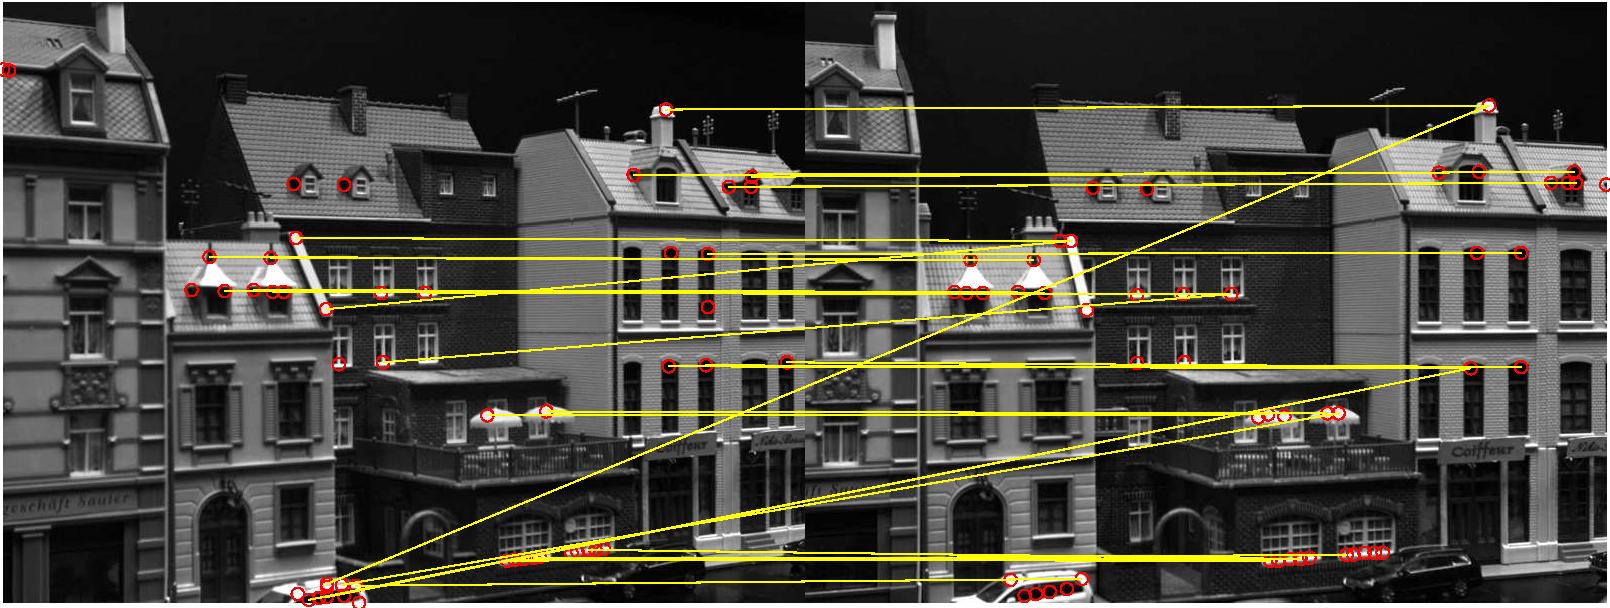
\includegraphics[width=\textwidth]{images/match_i1_i3_dog.pdf}
        \caption{DoG points matched between I1 and I3}
        \label{fig:i1_i3_dog}
    \end{subfigure}
\end{figure}
\begin{figure}[H]
    \begin{subfigure}[t]{\textwidth}
        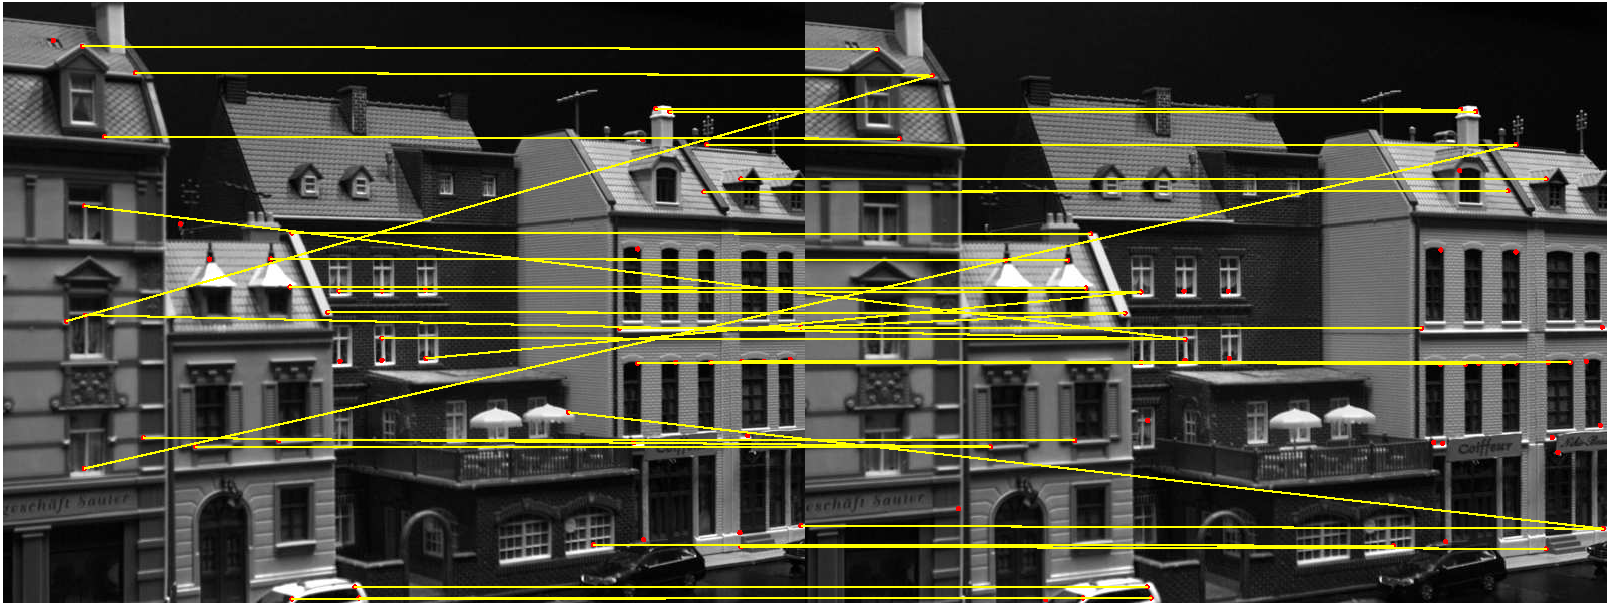
\includegraphics[width=\textwidth]{images/match_i1_i2_harris.pdf}
        \caption{Harris corners matched between I1 and I2}
        \label{fig:i1_i2_harris}
    \end{subfigure}
    \begin{subfigure}[t]{\textwidth}
        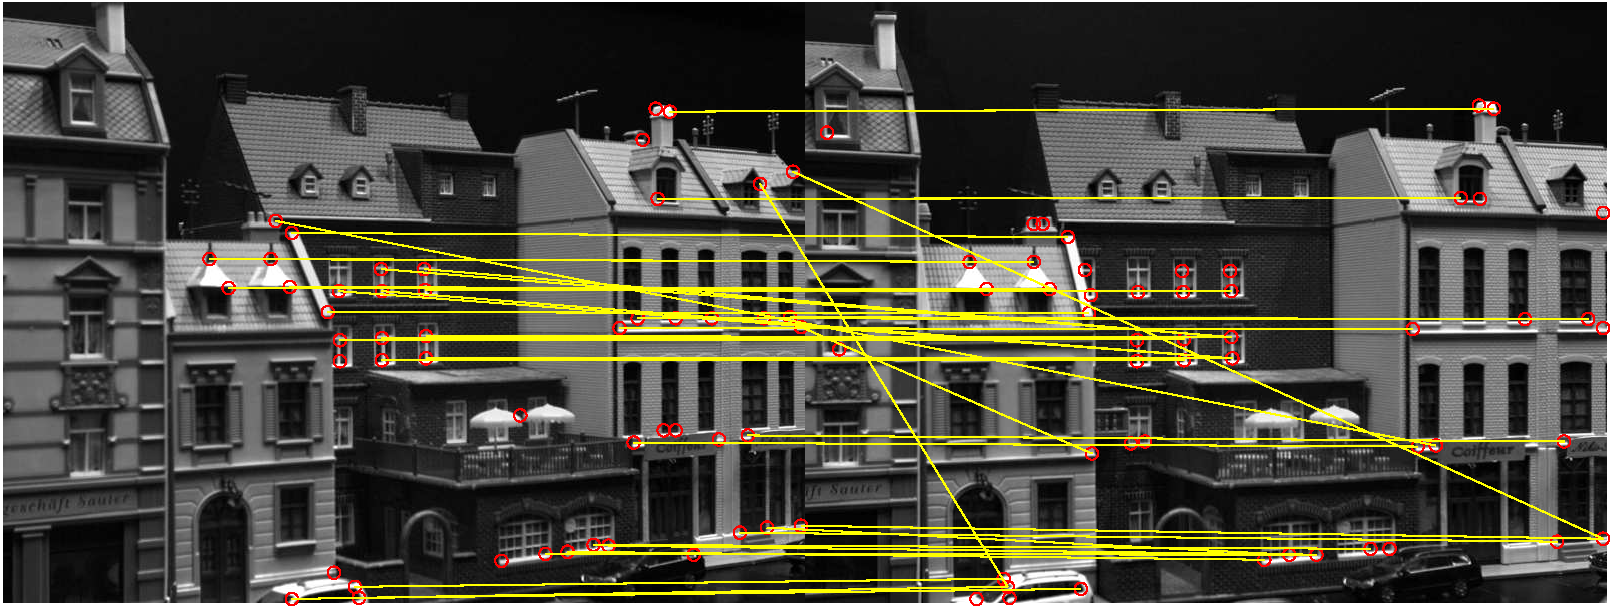
\includegraphics[width=\textwidth]{images/match_i1_i3_harris.pdf}
        \caption{Harris corners matched between I1 and I3}
        \label{fig:i1_i3_harris}
    \end{subfigure}
\end{figure}

\subsection{Normalized Cross Correlation}

The performance decreases since a larger variation in the view angle between
the two images naturally change the lighting and view of the physical objects.
This will in terms change the shapes captured by the camera. Furthermore some
previously captured interest points could be hidden due to the angle change
and new interest points could likewise be revealed. All these changes make it
harder for our matching algorithm as the optimal patch matches decrease in
similarity and hence we are prone to erroneous matching. Instead of using the
NCC similarity measure we could use a

\end{document}

